\chapter{Related Work}

In this chapter, some related work are illustrated in detail. Section \ref{relatpre} presents two previous theses and points out their deficiencies with regard to our problem. Section \ref{relatrec} introduces two recent models, PolygonRNN and Mask R-CNN. Section \ref{relatmot} gives the summary of these models and further discusses the feasibility of applying these models to our problem.

\section{Deep Learning Methods for Image Segmentation}\label{dlimgseg}

\section{Previous Theses}\label{relatpre}

There are two previous theses related to our problem, which are shown as follows.

\paragraph{Image Segmentation in Pixel Level}
In this thesis, our problem is treated as a pixel-wise image segmentation problem. The student employs a kind of deep neural network, U-Net, and make modification to classify each pixel in the aerial image as different labels, i.e. buildings, roads or background. The output of the model is a labelled mask. An example is shown in figure \ref{fig:egimgseg}. We can see that the model can well distinguish between buildings and roads. However, there are also some limitations in this method: (1) we do not know which pixel belongs to which building, meaning that there is no instance segmentation here; (2) the buildings cannot be detected unless we do further pixel connectivity detection; (3) there are no geometrical shapes of the objects. Therefore, this model cannot be fully used to solve our problems.

\paragraph{Rotated Bounding Box}
Another thesis utilizes the RPN (Region Proposal Network) part in Faster R-CNN and adds a branch for orientation degree. It predicts the rotated bounding boxes to `capture' each building instance in an aerial image. Thus, our problem here becomes a parameters regression problem, which aims at finding out the center coordinates, width, height, and the rotation degrees of the bounding box. The model used here is the modified RPN. The role of RPN part in original Faster R-CNN is to find RoIs (Regions of Interest), which are generally represented as bounding boxes or rectangles. This kind of representation can be very suitable for horizontal or vertical buildings. But we know that buildings are not always regular, many of them are inclined in the image. Therefore, in this thesis project, the RPN is modified and another branch for rotating the bounding boxes is added. This can make the boundary of the bounding box closer to the building. Figure \ref{fig:egrotbbox} shows an example output. We can see from the figure that each building instance can correspond to a rotated bounding box, and can be also limited tightly to the box. This methods can detect buildings very well, but the geometrical shapes found are limited to rectangles and cannot be more precise.

\begin{figure}[!h]
	\centering
	\subbottom[pixel-wise labelled mask\label{fig:egimgseg}]{
		\includegraphics[width=\figfig\textwidth]{2-00-0.png}
	}
	\subbottom[rotated bounding boxes\label{fig:egrotbbox}]{
		\includegraphics[width=\figfig\textwidth]{2-00-1.png}
	}
    \caption[Example outputs of two previous theses]{Example outputs of two previous theses. In (a), the pixels with red color refer to buildings, while the pixels with blue color refer to roads. In (b), each bounding box relates to one instance.}
	\label{fig:prethe}
\end{figure}

In short, the analysis and discussion of the two theses above show that although they have their own advantages and the effects are still good, they cannot fully reflect the geometrical shapes.

\section{Recent Models}\label{relatrec}

In this section, two recent models, PolygonRNN and Mask R-CNN are illustrated (see subsection \ref{relatpoly} and \ref{relatrcnn} respectively). PolygonRNN focuses on the segmentation of geometrical shape and the FPN (Feature Pyramid Network) in Mask R-CNN can be used for the detection of buildings.

\subsection{PolygonRNN}\label{relatpoly}
PolygonRNN aims at finding geometrical shape for an object instance, given the bounding box. The model is originally proposed for speeding up labeling the ground truth since it can achieve semi-automatic annotation of object instances, but the model can be used for single instance segmentation as well.

Most current methods regard the instance segmentation problem as a pixel-wise classification problem, generally labeling each pixel as object or background (see figure \ref{fig:egpxlmsk} for example). Different from this traditional way, the paper treats the segmentation task as a polygon prediction problem. In particular, PolygonRNN takes the image of instance as input and sequentially produces vertices of the polygon outlining the object (see figure \ref{fig:egpoly} for example).

\begin{figure}[!h]
	\centering
	\subbottom[an example building\label{fig:egorgimg}]{
		\includegraphics[width=\figfigfig\textwidth]{2-01-0.png}
	}
	\subbottom[per-pixel mask\label{fig:egpxlmsk}]{
		\frame{\includegraphics[width=\figfigfig\textwidth]{2-01-1.png}}
	}
	\subbottom[polygon representation\label{fig:egpoly}]{
		\frame{\includegraphics[width=\figfigfig\textwidth]{2-01-2.pdf}}
	}
    \caption[Comparison of pixel-wise mask and polygon]{Comparison of pixel-wise mask and polygon. (a) is the original image containing a building. (b) is the target mask of traditional pixel-wise instance segmentation, (c) is the desired prediction of polygon, of which the vertices are numbered.}
	\label{fig:egcmp}
\end{figure}

We know that predicting a polygon is equivalent to predicting each of its vertices. Thus, the paper regards polygon as a series of vertices, and uses RNN as the model to make coherent prediction. RNN is very powerful when data is related to time series as it can carry complex information about the history. In our case, the prediction of each vertex is dependent on the position of its two previous vertices. The paper also mentioned that another advantage over traditional methods is that RNN can capture the shape of the object even in ambiguous cases like shadows and saturation.

In short, we hope that PolygonRNN can be used to solve our problems, extracting geometric shapes of buildings in aerial images, since the buildings in such images can be also regarded as polygons. For more details of the architecture, please refer to section \ref{modpoly}.

\subsection{Mask R-CNN}\label{relatrcnn}

Mask R-CNN is a general framework for object instance segmentation. It is the latest model in the R-CNN family, which includes R-CNN, Fast R-CNN, Faster R-CNN as well. Mask R-CNN can efficiently detect objects in an image and generate a high-quality segmentation mask for each instance simultaneously. Figure \ref{fig:rcnnres} shows example results of Mask R-CNN. We can see from the figure that this model achieves excellent results. Figure \ref{fig:rcnnsimmod} shows the simplified structure of Mask R-CNN. Each part of the structure are illustrated as follows.

\begin{figure}[!h]
	\centering
	\includegraphics[width=\fig\textwidth]{2-02.pdf}
    \caption[Example results of Mask R-CNN]{Example results of Mask R-CNN.}
    \label{fig:rcnnres}
\end{figure}
\begin{figure}[!h]
	\centering
	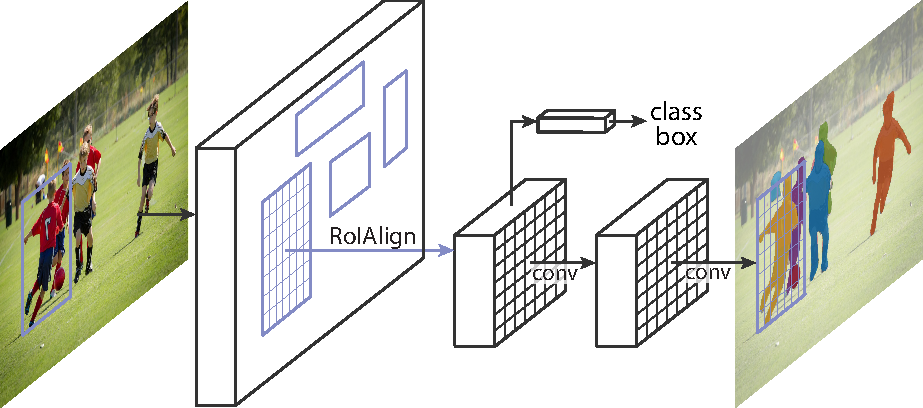
\includegraphics[width=\fig\textwidth]{2-03.pdf}
    \caption[Simplified model structure of Mask R-CNN]{Simplified model structure of Mask R-CNN. Feature Pyramid Network locates at the first layer in the figure.}
    \label{fig:rcnnsimmod}
\end{figure}

\paragraph{Feature Pyramid Network} The original image is first passed through the FPN (Feature Pyramid Network), which locates at the first layer in figure \ref{fig:rcnnsimmod}. Just like the RPN mentioned in section \ref{relatpre}, FPN is also a kind of network for finding RoIs. Actually, FPN is an upgraded version of RPN used in both Faster R-CNN and the previous thesis. Compared with RPN, FPN solves the problem of multi-scale detection and introduces feature pyramid, and thus improves the accuracy of detection, especially for small objects in the image.

\paragraph{Classification Branch}
The classification branch exists from the earliest R-CNN to the present Mask R-CNN.  It classifies each object in RoI found by FPN as different classes and gives probability, using fully connected layers. However, this branch is not relevant to our problem, since currently we only interested in buildings rather than kinds of different objects in an aerial image.

\paragraph{Mask Branch}
Mask R-CNN extends Faster R-CNN by adding the mask branch for predicting an object mask on each RoI in parallel with the existing classification branch. This branch uses small FCN (Fully Convolutional Network) for the pixel-wise semantic segmentation. The mask branch should be relevant to our problem, but the mask it predicts is still in the pixel level instead of polygon.

In short, Mask R-CNN can surpass prior instance segmentation results, but it cannot give any geometrical information of the objects in an image. Therefore, FPN is the only part of Mask R-CNN, which can be utilized to solve our problems. We hope that FPN can make correct detection of all buildings and localizing each using a bounding box. For more details of the architecture of FPN, please refer to section \ref{modfpn}.

\section{Motivation}\label{relatmot}
Table \ref{tab:summod} makes a summary for all models mentioned in sections \ref{relatpre} and \ref{relatrec}. From the table we can conclude that none of these models meets our requirements. Thus, combination of two or even more models becomes necessary.

\begin{table}[!h]
	\centering
	\caption[Summary of Related Models]{Summary of Related Models.}
	\label{tab:summod}
	\begin{tabular}{l|l|l|l}
	\hline
	Model & Localization & Geometrical Shape & Classification \\ \hline
	Modified U-Net & Limited\tablefootnote{As mentioned in section \ref{relatpre}, localization requires further pixel connectivity detection.} & No & \textbf{Yes} \\
	Modified RPN & \textbf{Yes} & Limited\tablefootnote{As mentioned in section \ref{relatpre}, only rotated bounding boxes are found.} & No \\
	PolygonRNN & No & \textbf{Yes} & No \\
	Mask R-CNN & \textbf{Yes} & No & \textbf{Yes} \\
	FPN & \textbf{Yes} & No & No \\
	What We Want & \textbf{Yes} & \textbf{Yes} & N/A \tablefootnote{As mentioned in section \ref{prodef}, segmentation of roads is currently not considered in our project, thus the cell here shows `N/A'.} \\
	\hline
	\end{tabular}
\end{table}

After observation, we propose a possible approach, simply replacing the mask branch in Mask R-CNN with PolygonRNN so that the modified model can predict polygon rather than pixel-wise mask for each RoI. This model takes advantages from both models, thus it can be applied to our problem. In practice, we just combine FPN and PolygonRNN and name it a new model \modelnameshort\ (\modelnamelong), of which the architecture is shown in detail in section \ref{modmer}.
